\documentclass{article}
\usepackage[utf8]{inputenc}
\usepackage{blindtext}
\usepackage{graphicx}
\usepackage{amsmath}
\usepackage{csvsimple}
\usepackage{pdfpages}
\usepackage{hyperref}
\usepackage{gensymb}

\begin{document}
\begin{center}
\textbf{\Huge{University of South Bohemia}}\\
\vspace{50px}
\textbf{\Large{Faculty of Science}} \\
\vspace{30px}
\includegraphics[width=120px]{~/school/logo.png} \\
\vspace{30px}
\textbf{\large{Praktika III}}
\vspace{20px}
\\
\vspace{20px}
\large{Frank-Hertzův experiment} \\
\vspace{60px}
\end{center}
\begin{flushleft}
Datum: 18.8.2023 \\
Jmeno: Martin Skok \\
Obor: Fyzika \\
Hodnoceni:
\end{flushleft}
\newpage
\section{Úkoly}
\subsection{}
Proměřit voltampérovou chrakteristiku Franck-Hertzovy trubice (triody) plněné
rtuťovými parami a určit energii přechodu v atomu rtuti.
\subsection{}
Proměřit voltampérovou chrakteristiku Franck-Hertzovy trubice (tetrody) plněné
neonem a určit energii přechodu v atomu neonu.
\subsection{}
Přepočíst zjištěné hodnoty energií $\Delta E [eV]$ na vlnočet $\nu [cm^{-1}]$ a po porovnání
se spektroskopickými tabulkami určit atomové orbitaly účastnící se naměřených energetických
přechodů v atomech rtuťi a neonu.
\section{Pomůcky}
Franck-Hertzova trubice plněná rtuťovými parami, Franck-Hertzova trubice plněná neonem,
napájecí zdroj, zařízení 3BNETlog, počítač s aplikací 3BNETlog a propojovací vodiče.
\section{Teorie}
\section{Postup měření}
\subsection{Trubice s rtuťí}
Nejdříve bylo zkontrolováno zapojení obvodu.
Lampa se zahřála na $210 ^{\circ} C$. Byl zapnut počítač a bylo do něj připojeno zařízené 3BNETlog.
V počítačí se otevřel program 3BNETlab. V softwaru se nastavily potřebné parametry.
Nastavil jsem žhavící napětí na $6,5 V$ a postupně jsem zvedal urychlovací napětí na $20V$.
Na osciloskopu se objevily dvě křivky: modrá (uychlovací napětí) a červená (proud na anodě).
Urychlovací napětí jsem zvyšoval až na hodnotu $80V$.
Všechna data jsem potom exportoval.
\subsection{Trubice s neonem}
Zapojil jsem neonovou trubici podle návodu.
Zapojil jsem jí do počítače a zapnul zase stejný software.
Nastavil jsem parametry podle návodu.
Nastavil jsem řídící napětí na $9V$ a urychlující napětí na $80V$.
Zvyšoval jsem žhavící napětí, dokud se neobjevil oranžový plamen v trubici.
Na osciloskopu se objevili dvě křivky jako posledně.
Zvyšoval jsem zpomalující napětí, dokud nebyla křivka téměř rovná.
Potom jsem opět upravil parametry tak, aby bylo na křivce dobře rozeznat extrema.
Data jsem exportoval.
\section{Vypracovaná data}
\subsection{Grafy}
\begin{figure}[!h]
  \hspace*{-10em}
  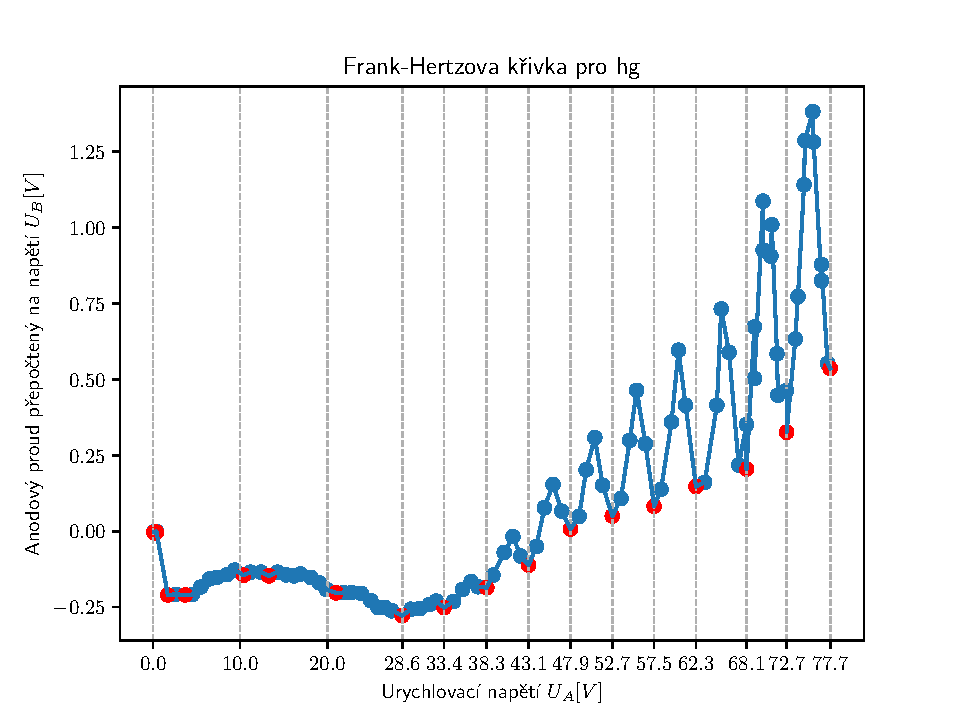
\includegraphics[scale=1.2]{data/hg.pdf}
  \caption{Frank-Hertzova křivka pro rtuť}
\end{figure}
\begin{figure}[!h]
  \hspace*{-10em}
  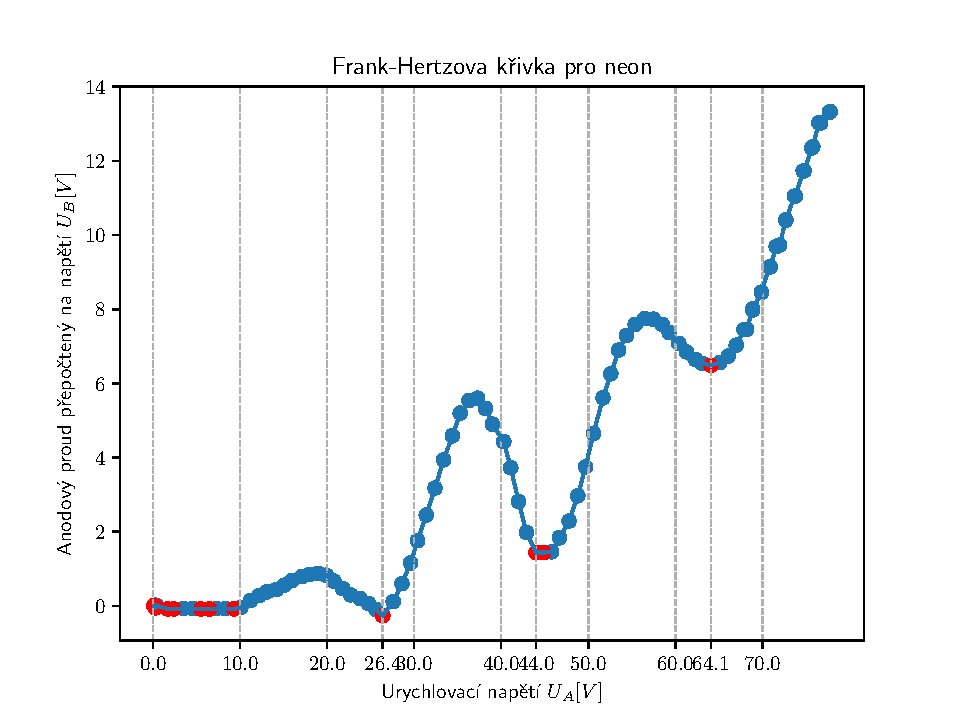
\includegraphics[scale=1.2]{data/neon.pdf}
  \caption{Frank-Hertzova křivka pro neon}
\end{figure}
\newpage
\subsection{Tabulky}
\footnotesize{Tabulka 1: rtuť}\\
\csvreader[
tabular = |c|c|c|,
table head =
\hline
{index} & {Peaky černých pixelů} & {Vzdálenost mezi}\\
\hline
\hline,
late after line = \\\hline
]{data/hg.csv}{}{
  \csvcoli & \csvcolii & \csvcoliii}
\\
\vspace{1em}
\\
$\overline{\Delta U_{Hg}} = 4.463$\\
$\sigma_{\Delta U}_{Hg} = 0.456$
\\
\vspace{1em}
\\
\footnotesize{Tabulka 2: neon}\\
\csvreader[
tabular = |c|c|c|,
table head =
\hline
{index} & {Peaky černých pixelů} & {Vzdálenost mezi}\\
\hline
\hline,
late after line = \\\hline
]{data/neon.csv}{}{
  \csvcoli & \csvcolii & \csvcoliii}
\\
\vspace{1em}
\\
$\overline{\Delta U_{Ne}} = 12.56$\\
$\sigma_{\Delta U}_{Ne} = 6.324$
\\
\vspace{1em}
\\
Chybu jsem počítal podle vzorce
$$\sigma_{U} = \sqrt{\frac{ \Sigma_{i=1}^{i=n}(\overline{U}-U)^{2} }{n(n-1)} }$$
\vspace{2em}
Po přenásobení těchto hodnot elementárním nábojem mi vyjde energie, kterou elektrony ztrácejí při srážkách mezi atomy.
$$E_{hg} = e \cdot \Delta U_{Hg} = 7,1515 \cdot 10^{-19} [J]$$
$$E_{ne} = e \cdot \Delta U_{Ne} = 2,0133 \cdot 10^{-18} [J]$$
\\
Tyto hodnoty jsem pak přepočetl na vlnočet pomocí vzorce
$$\nu = \frac{E}{hc} [m^{-1}]$$
Po dosazení do vzorce mi vyšlo
$$\nu_{Hg} = 3,6 \cdot 10^{6}$$
$$\nu_{Ne} = 10,13 \cdot 10^{6}$$
\newpage
Chybu vlnočtu jsem počítal jako
$$\delta_{Hg} = \sqrt{ \left(  \frac{ \partial \left( \frac{e \cdot E_{Hg}}{c \cdot h} \right) }{ \partial (h \cdot c) } \cdot \sigma_{E}_{Hg}  \right)^{2} }$$
$$\delta_{Hg} = \sqrt{ \left( \frac{c \cdot E_{Hg} + c \cdot h}{h^{2} c^{2}} \sigma_{E}_{Hg} \right)^{2} }$$
$$\delta_{Hg} = $$


\end{document}
